\chapter{Introducción}

    El diseño de los sistemas de señalamiento es un proceso complejo que involucra, principalmente, tres etapas: el análisis de la red ferroviaria, la detección de zonas de mayor probabilidad de descarrilamientos y colisiones, y la óptima localización de las señales correctas para cada función [REF]. La generación automática del señalamiento es de gran importancia y utilidad para el desarrollo de redes ferroviarias nuevas o para revitalizar redes ferroviarias abandonadas o en desuso. Es relevante incluso en redes ferroviarias que son alteradas debido a la adición, modificación o eliminación de elementos ferroviarios tales como pasos a nivel o plataformas, lo cual implica que el señalamiento debe actualizarse en consecuencia.
    
    En este trabajo presentamos una herramienta capaz de automatizar el diseño del señalamiento y la implementación del sistema de enclavamiento ferroviario para cualquier locación, dado únicamente el diseño de su traza ferroviaria. Se discutirán los detalles del diseño de la herramienta, su arquitectura, casos de uso y aplicaciones en locaciones teóricas y reales.

\section{Topologías ferroviarias}
    \label{sec:topologias}
    Las redes ferroviarias presentan dos piezas fundamentales en su infraestructura: su topología y los elementos ferroviarios que la componen. La topología es el entramado de vías férreas, cuyo diseño busca cumplir una función particular, interconectando diversos elementos ferroviarios. Los elementos ferroviarios pueden ser para determinar la ubicación del tren, para delimitar la circulación de vehículos en cruces ferroviarios, permitir el ascenso y descenso de pasajeros, o para modificar dinámicamente los caminos por los que los trenes circulan, entre otras funciones \cite{Paper_4,Paper_13,Paper_17,Paper_175}

    Muchos de los elementos ferroviarios inciden en la circulación del tren, por lo que el conductor debe ser informado de su estado. Es tarea del señalamiento ferroviario alertar a los conductores ferroviarios de cualquier elemento que pueda representar un peligro, evitando así colisiones con otras formaciones o descarrilamientos en zonas críticas \cite{Paper_168,Paper_176,Paper_202,Paper_203}. 
    
    El señalamiento ferroviario incluye un elemento fundamental: los semáforos ferroviarios, de ahora en adelante denominados "señales". Las señales informan al conductor de la habilitación o denegación de uso de las vías posteriores mediante su color, denominado aspecto. Cada señal puede presentar un único aspecto por vez de un conjunto posible que varía según el país o la región. Los aspectos utilizados en Argentina son el verde (permitido avanzar), amarillo (atención) y rojo (detenerse) \cite{RITO}. Algunas señales pueden no tener el aspecto verde (señales de maniobras de dos aspectos) o incorporar un aspecto extra entre el rojo y el amarillo (señales de cuatro aspectos que incluyen el doble amarillo).
    
    Dos señales consecutivas con la misma dirección y sentido constituyen una ruta ferroviaria \cite{RITO,INTERLOCKING_BASIC,IRSE}. Los operarios ferroviarios solicitan al sistema de enclavamientos las rutas que necesitan de acuerdo con la logística deseada. El sistema de enclavamientos habilitará o denegará las rutas solicitadas en función del estado de los elementos ferroviarios cercanos y de las demás rutas activas. Esta función es vital para el sistema ferroviario y su fin último es permitir la circulación de trenes de forma segura o, de no ser posible, no permitir circulación alguna \cite{Paper_175,Paper_176,INTERLOCKING_BASIC,IRSE}.

	En las siguientes subsecciones, se describen algunas de las topologías ferroviarias más ampliamente utilizadas.
	
    \subsection{Derivación ferroviaria}

Cuando es necesario interconectar dos puntos separados por una distancia de decenas o cientos de kilómetros donde hay poco tráfico ferroviario, resulta económicamente poco conveniente construir vías en ambos sentidos. No obstante, construir una sola vía bidireccional presenta inconvenientes logísticos notorios: una formación que circule entre los puntos A y B excluye a cualquier formación que quiera circular de B a A sin colisionar. %No sería posible utilizar la infraestructura en el sentido opuesto mientras se encuentre ocupada.

La solución mas utilizada emplea islas de enclavamiento a modo de bypass cada cierta cantidad de kilómetros, como se ilustra en la Figura \ref{fig:bypass_1}. Estas islas permiten que las formaciones puedan cruzarse sin riesgo de colisión. La primer formación en llegar a la isla de enclavamientos accede al bypass por la vía superior y espera a que la formación en sentido contrario circule por la vía inferior. Una vez despejado el camino que resta por recorrer, la formación reingresa a la vía principal y retoma su marcha.

    \begin{figure}[h]
        \centering
        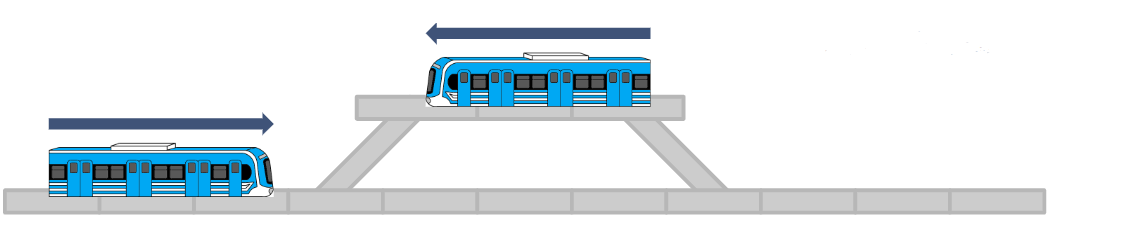
\includegraphics[width=1\textwidth]{Figuras/bypass}
        \centering\caption{Topología de derivación ferroviaria.}
        \label{fig:bypass_1}
    \end{figure}
    
Las topologías de derivación ferroviaria se utilizan principalmente para transportar materias primas entre locaciones rurales a grandes distancias de los puestos. Es deseable tanto una logística óptima, para transportar mas bienes y mas rápido, cómo un sistema seguro que garantice que los bienes lleguen a destino.
    \subsection{Simple}

En entornos urbanos donde las estaciones ferroviarias se encuentran separadas entre sí por unos pocos kilómetros es necesaria una interconectividad mayor. El sistema ferroviario debe satisfacer la demanda de una población mayor y a la vez coexistir con un trazado vehicular mucho mas denso que cruza al trazado ferroviario en varios puntos. En este contexto, una topología simple como la presentada en la Figura \ref{fig:simple_1} es una solución óptima al problema planteado.

    \begin{figure}[h]
        \centering
        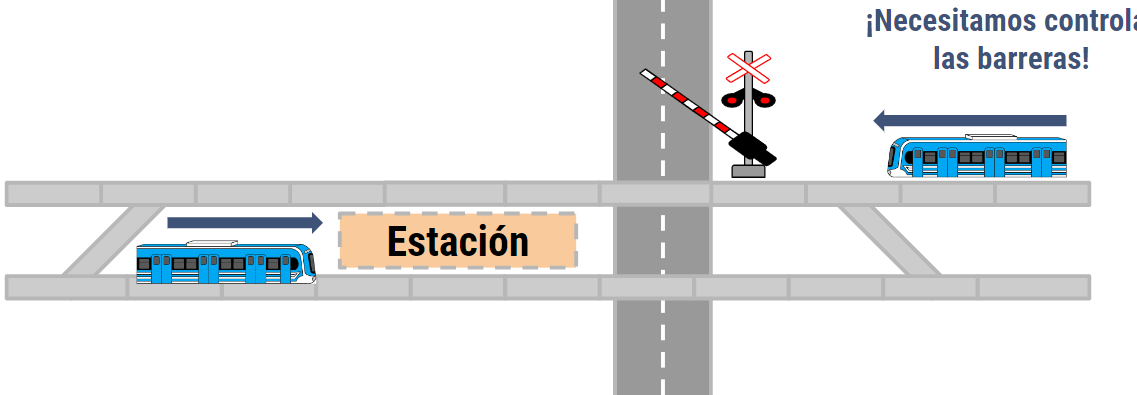
\includegraphics[width=1\textwidth]{Figuras/simple}
        \centering\caption{Topología simple.}
        \label{fig:simple_1}
    \end{figure}

El cruce entre el trazado ferroviario y el trazado vehicular se denomina paso a nivel. El sistema de enclavamientos deberá garantizar que el paso a nivel se encuentre despejado de vehículos y peatones antes de permitir la circulación de trenes sobre el mismo. Esto se logra mediante el uso de una barrera ferroviaria, un mecanismo que mantiene la barrera en alto mientras no se detecten formaciones en las proximidades del paso a nivel.

Las topologías simples suelen contar con dos vías unidireccionales en sentido ascendente y descendente. 
Las vías ascendentes son aquellas por las que las formaciones circulan en la dirección del kilometraje creciente. Mientras que las vías descendentes son aquellas por las que circulan en la dirección del kilometraje decreciente [REF]. El kilómetro cero es la estación principal de la línea ferroviaria, como por ejemplo: Plaza Constitución (Línea Roca), Once de Septiembre (Línea Sarmiento) o Retiro (Línea Mitre y Linea San Martín). Las formaciones pueden cambiar de vía ascendente a descendente, o viceversa, utilizando un cambio ferroviario.
    \subsection{Hub}

A medida que mas líneas ferroviarias coexisten en la misma red se vuelve inevitable que varias líneas compartan la misma estación utilizando diferentes plataformas en paralelo. Con una logística mas flexible, las diferentes líneas incluso pueden utilizar de forma alternada las mismas plataformas y, por lo tanto, las mismas vías principales. Además, es necesario contar con mecanismos para retirar trenes de la red para su mantenimiento y volver a inyectarlos a la red cuando la demanda aumente. Esto se logra por medio de talleres ferroviarios en las inmediaciones de las estaciones que actúan como un hub ferroviario. La topología de hub ferroviario se ilustra en la Figura \ref{fig:hub_1}.

    \begin{figure}[h]
        \centering
        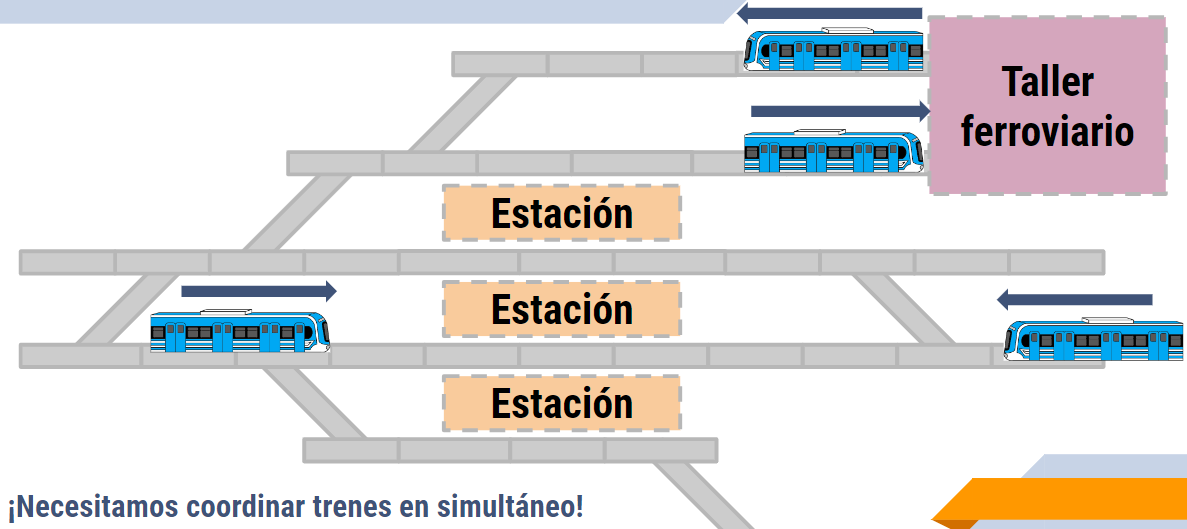
\includegraphics[width=1\textwidth]{Figuras/hub}
        \centering\caption{Topología hub.}
        \label{fig:hub_1}
    \end{figure}
    
Las tareas del sistema de enclavamientos van aumentando en complejidad a medida que se suman nuevos actores. Debe coordinar diversas formaciones de distintas líneas, accediendo a diferentes plataformas, cumpliendo diferentes horarios de arribo y partida. A su vez, debe asegurarse de que las formaciones circulen con seguridad pero sin descuidar la puntualidad. Adicionalmente, debido a que la demanda varía a lo largo del día, deberá tener flexibilidad para inyectar nuevas formaciones a la red o remover las que presenten desperfectos técnicos. Todas estas acciones deben realizarse en simultáneo y en un entorno de alto dinamismo.
    \subsection{Estación Terminal}

Las estaciones terminales presentan una gran cantidad de vías principales y plataformas en paralelo, en las cuales confluyen una o varias líneas ferroviarias. A diferencia de estaciones de tipo hub que pueden presentar finales de vía relativos, las estaciones terminales poseen finales de vía absolutos. Es decir, las formaciones que circulan por la vía descendente deberán detener su marcha completamente antes de llegar al fía de vía, para luego retomar su marcha en sentido contrario, por la vía ascendente. Esta operación puede realizarse de manera inmediata en formaciones con locomotras eléctricas en ambos extremos del tren o con locomotoras diesel luego de varias maniobras que requieren el uso de diversos cambios de vías. En la Figura \ref{fig:terminal_1} se ilustra un ejemplo de una estación terminal.

    \begin{figure}[h]
        \centering
        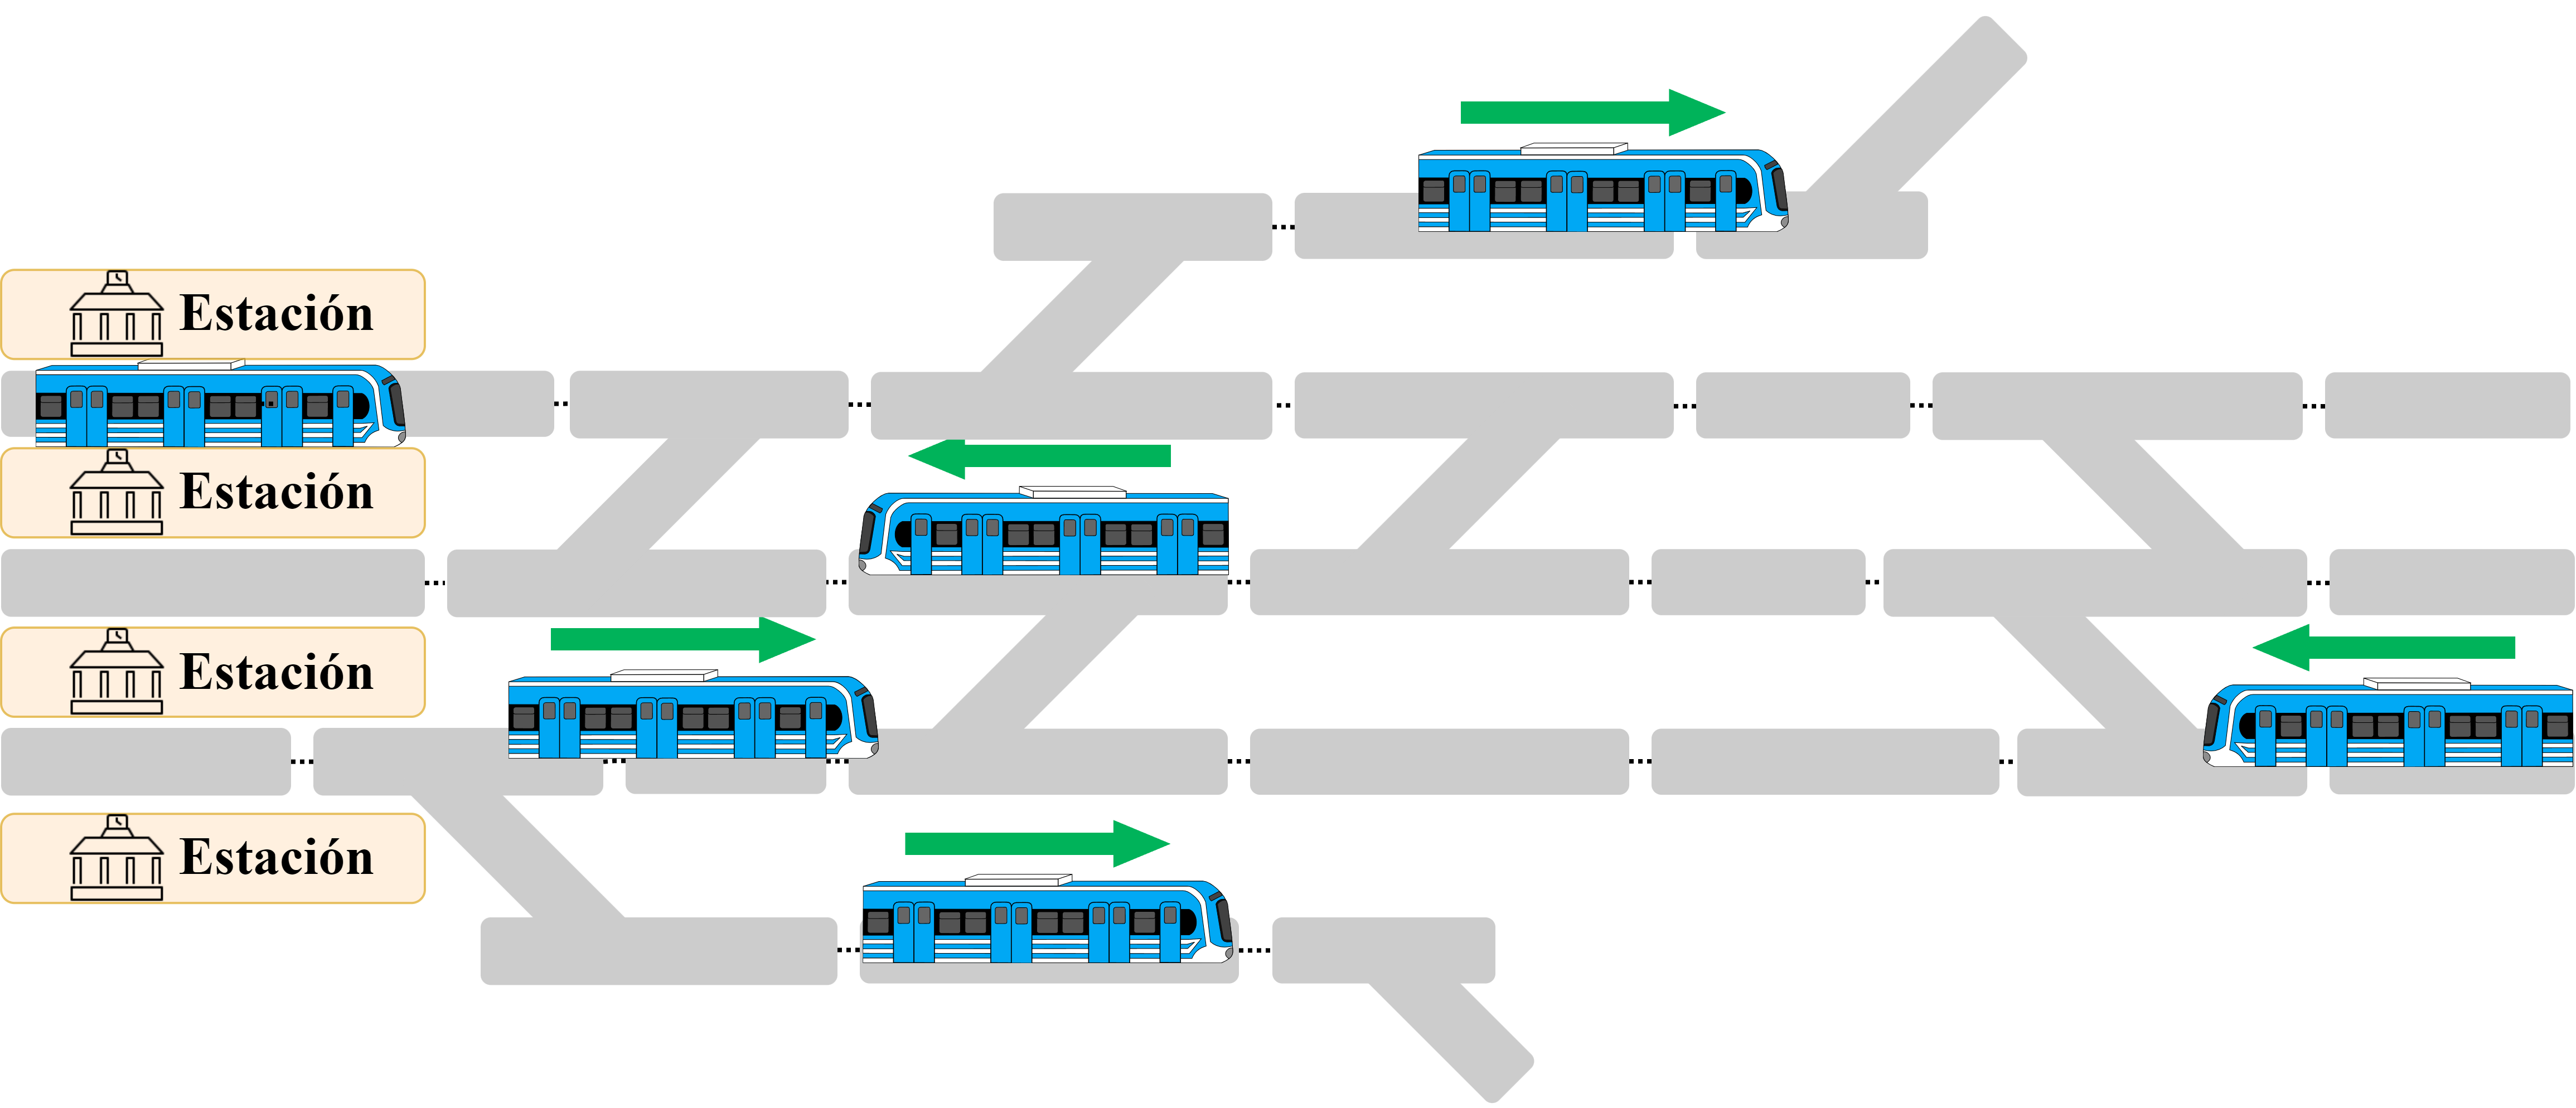
\includegraphics[width=1\textwidth]{Figuras/terminal}
        \centering\caption{Topología terminal.}
        \label{fig:terminal_1}
    \end{figure}

En las estaciones terminales suelen confluir la información en tiempo real de la terminal y las estaciones mas próximas de la línea, o incluso la información en tiempo real de la totalidad de la línea. Esta característica, además de ser la estación de mayor tamaño de la línea, les otorga una jerarquía tal que suelen concentrar parcial o totalmente el control del señalamiento de la red. Las decisiones tomadas en una estación terminal tienen un gran impacto en el sistema de transporte de toda la línea, directa o indirectamente. Estas operaciones deben considerar cientos o miles de estados en simultáneo, por lo que ejecutarlas de forma manual es muy complejo o incluso imposible. Un sistema de enclavamientos moderno, robusto, que pueda garantizar una altísima disponibilidad, mantenibilidad y seguridad es indispensable para llevar a cabo estas tareas.
\section{Estado del arte}

\lipsum[1]

\subsection{Empresas del sector ferroviario}

\lipsum[1]
\subsection{Herramientas existentes}

\lipsum[1]
\subsection{Estudios realizados}

\lipsum[1]
\subsection{Enfoque funcional vs enfoque geografico}

\lipsum[1]

\subsection{RailTopoModel}

\lipsum[1]

\subsubsection{Modelo de grafos}

\lipsum[1]
\subsubsection{Topología y niveles}

    La topología del modelo es una parte fundamental del estándar. RailTopoModel incluye el "principio de agregación", por el cual los elementos pueden ser agrupados en entidades mas grandes. En la Figura \ref{fig:RTM_1} se puede visualizar la estructura de capas propuesto por RailTopoModel.

    \begin{figure}[!h]
        \centering
        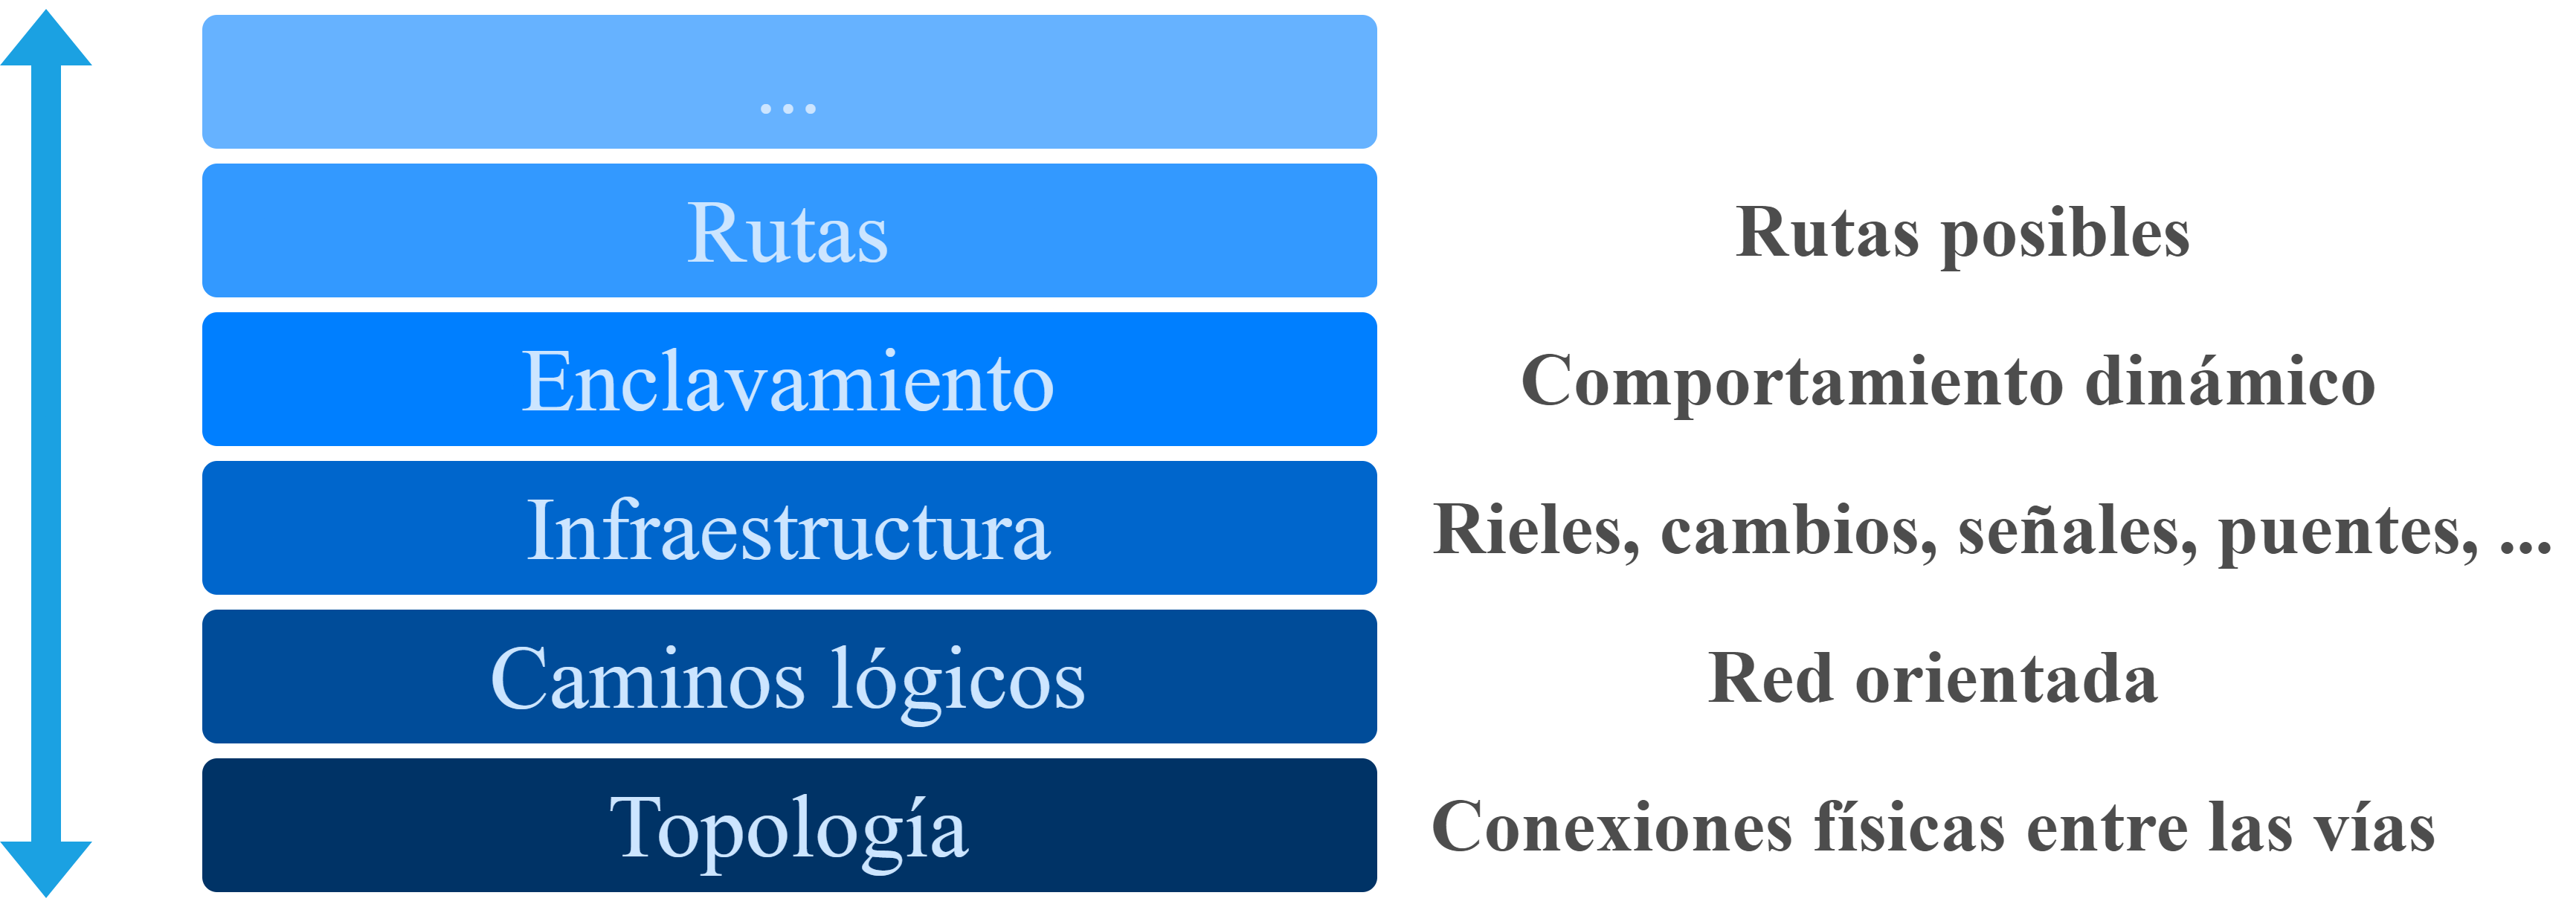
\includegraphics[width=1\textwidth]{Figuras/capas}
        \centering\caption{Estructura de capas de RailTopoModel.}
        \label{fig:RTM_1}
    \end{figure}
    
    La topología de la red está compuesta por los nodos (netElements) y las aristas (netRelations) que los conectan entre sí, lo cual constituye el nivel microscópico de la red. Cada nodo representa un tramo de vías que puede tener ciertos elementos ferroviarios asociados o ninguno. A su vez, los nodos pueden ser agrupados en diversos caminos lógicos, que son el conjunto de nodos cuyas relaciones y navegabilidad les permite constituir un camino físico entre ellos.

    A medida que se agrupan mas y mas cambios de vías junto con las plataformas y máquinas de cambios se constituye un punto de operación. La descripción en base a puntos de operación es a nivel mesoscópico, como se muestra en la Figura \ref{fig:RMT_2}, y es utilizado en logística. Las secciones de vía que no incluyen plataformas en las cuales las formaciones puedan detenerse se denominan secciones de líneas, o simplemente "líneas" dentro del modelo de RailTopoModel. La descripción que incluye tanto los puntos de operación como las secciones de líneas es a nivel macroscópico. Esta simplificación de la red es de gran importancia, ya que es ampliamente utilizada en los mapas ferroviarios de todas las estaciones del mundo: los puntos de operación son las estaciones y las secciones de línea son las vías que las comunican. 
    
    \begin{figure}[!h]
        \centering
        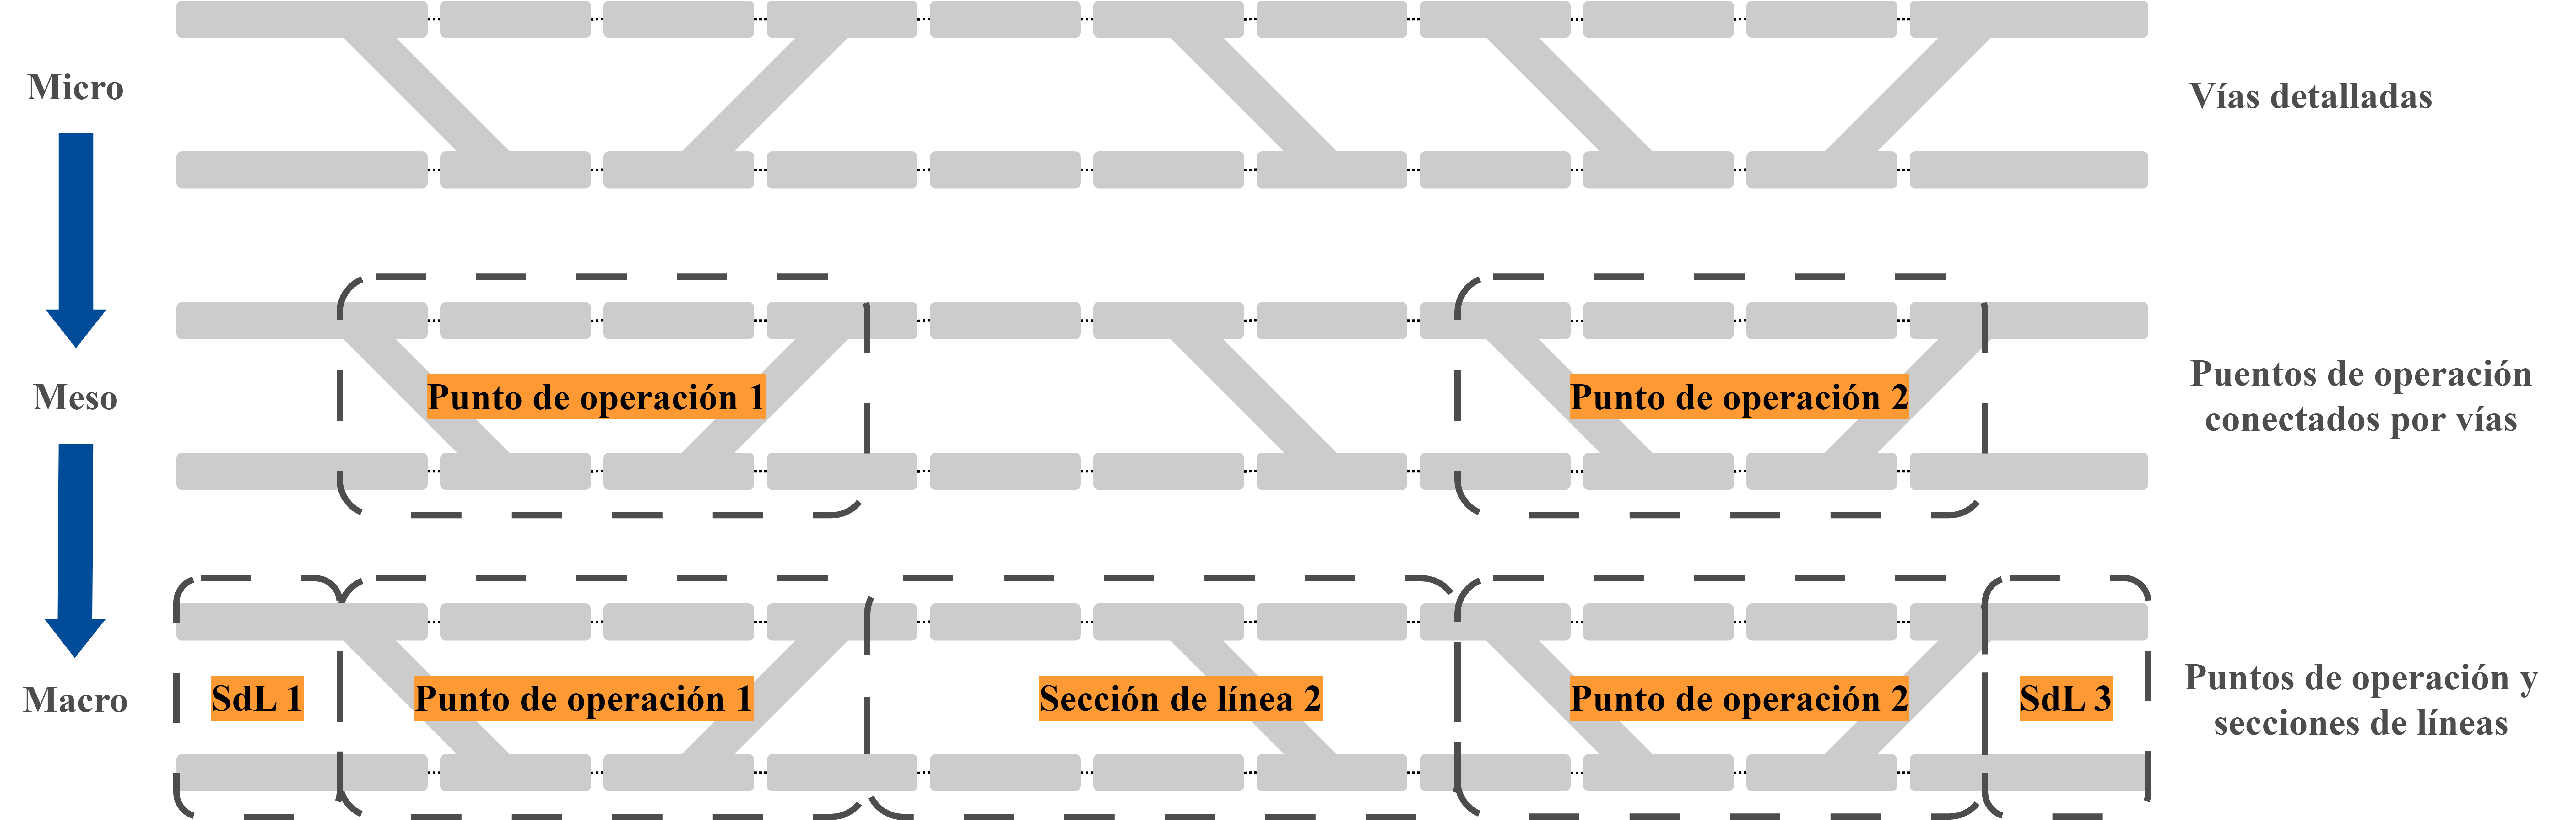
\includegraphics[width=1\textwidth]{Figuras/railtopomodel}
        \centering\caption{Niveles microscópico, mesoscópico y macroscópico.}
        \label{fig:RTM_2}
    \end{figure}
    
    Las instalaciones y sus propiedades constituyen todos los elementos ferroviarios asociados a un nodo. Estos representan elementos físicos del mundo real, pueden ser estáticos o dinámicos. Los elementos estáticos como los puentes, curvas y estaciones no alteran sus propiedades en ningún momento. Los elementos dinámicos como los pasos a nivel, máquinas de cambios o señales tienen algunas propiedades fijas, como la posición física del elemento, pero otras variables, como la posición mecánica de alguna de sus piezas o el estado eléctrico de sus circuitos.

    Un sistema de enclavamiento relaciona todos los módulos previamente mencionados. El sistema de enclavamientos modificará el estado de los elementos dinámicos, basados en el estado actual de los mismos, sometido a las restricciones impuestas por los elementos estáticos, buscando habilitar los caminos lógicos mas cortos y seguros entre un punto A y B.

    Finalmente, en base al estado de los elementos dinámicos decidido por el sistema de enclavamiento, buscando el camino óptimo entre A y B que no comprometa la infraestructura del sistema, es que obtenemos las rutas permitidas. Todas las restricciones impuestas por las capas inferiores (caminos lógicos posibles, limitaciones de la infraestructura o estados previos que sean incompatibles con lo pedido) terminan emergiendo como un conjunto de rutas posibles de ser utilizadas, en detrimento de otras que, en ese instante de tiempo, no podrán ser habilitadas hasta que el estado del sistema se modifique.

    Como se puede apreciar, en este modelo, las rutas son una consecuencia de la infraestructura que se tiene y de los estados anteriores del sistema, producto de las rutas previamente pedidas. Un análisis completo de la topología e infraestructura permitiría obtener todo el conjunto de rutas posibles, para cualquier estado alcanzable por el sistema.
\subsection{RailML}
    \label{sec:railML}
    
    railML [REF] (del inglés, Railway Markup Language) es un estándar abierto de comunicación de datos entre herramientas ferroviarias desarrollado por las principales empresas de la industria ferroviaria a partir del año 2002. Las primeras dos versiones del estándar se diseñaron en base al enfoque funcional, pero en 2017 se lanzó railML 3.0, basado en RailTopoModel y, por lo tanto, adoptando un enfoque puramente geográfico.

\subsubsection{RailML 3.0}

\lipsum[1]
\subsubsection{Uso del estándar railML en la industria ferroviaria}

    El estándar railML es promovido por empresas de gran peso en la industria ferroviaria como Siemens, Thales, Alstom, CAF, ADIF y Toshiba, que concentrán la mayoría de la cuota de mercado global [REF]. Adicionalmente, diversas instituciones y organismos ferroviarios a nivel estatal y nacional hacen uso del estándar railML en sus desarrollos ferroviarios [REF], tales como: Queensland Rail, Transdev Deutschland, Transperth, Saudi Railway Company y Transport for New South Wales, entre otras.

    En sus primeros años de vida railML experimentó varios cambios, pero no fue hasta su versión 3.0 con enfoque geográfico que el uso del estándar creció exponencialmente. Entre el 40 y el 60\% de sus usuarios adoptaron el estándar en los últimos siete años [REF].

    Podemos encontrar las herramientas mas diversas basadas en railML: analizadores de infraestructura [MAPREX], planificador logístico para material rodante [IVU], visualizadores de datos [railViVid], planificadores de infraestructura [VIS ALL 3D] y visualizadores/simuladores de infraestructura enclavamiento [D4R]. Muchas de ellas certificadas e intercompatibles entre sí. Aunque la mayoría son herramientas de código cerrado, el estándar railML es abierto y sigue un principio bottom-top: todas las necesidades de la industria son tenidas en cuenta para ser incorporadas en nuevas versiones del estándar, siguiendo el exitoso modelo del estándar USB, Bluetooth y GSM. 
\section{Contexto de nuestro grupo de investigación y los trabajos realizados}

    Argentina continúa utilizando mayormente sistemas de enclavamiento mecánicos o electromecánicos de mediados dedl siglo XX [REF], mientras que otros países han actualizado sus sistemas de transporte de cargas y pasajeros con electrónica de última generación. La falta de mantenimiento adecuado y obsolesencia tecnológica impacta negativamente en la seguridad que dichos sistemas pueden brindar a los pasajeros, a la carga que transportan y/o a la infraestructura que utilizan.

    Adicionalmente, los sistemas de enclavamiento son en su totalidad importados y muy costosos, fabricados por una docena de empresas a nivel mundial, lo cual restringe la competencia y por lo tanto la variedad de precios es limitada. Un sistema de enclavamientos completo puede costar mas de 10 millones de dólares [REF], pero no se necesita solamente uno sino dececnas de ellos para modernizar toda la zona metropolitana de buenos Aires.

    En este contexto, en 2015 se creó el CONICET-GICSAFe [REF], cuyas siglas corresponden al Grupo de Investigación en Calidad y Seguridad de las Aplicaciones Ferroviarias, conformado por docentes e investigadores de una decena de universidades e instituciones públicas argentinas. El grupo desarrolló sistemas electrónicos e informáticos para aplicaciones ferroviarias relacionadas con la seguridad, a partir de la generación de un prototipo funcional y la documentación correspondiente que luego se transfirió siempre en su totalidad a Trenes Argentinos [REF], que es la Sociedad del Estado que opera las líneas Roca, Sarmiento, Mitre, San Martín y Belgrano Sur, entre otras. En la Figura \ref{fig:contexto} se ilustran todos los logros e hitos alcanzados por GICSAFe en relación con el desarrollo de un sistema de enclavamientos desde 2018 y los objetivos a futuro hasta 2025.

    \begin{figure}[h]
        \centering
        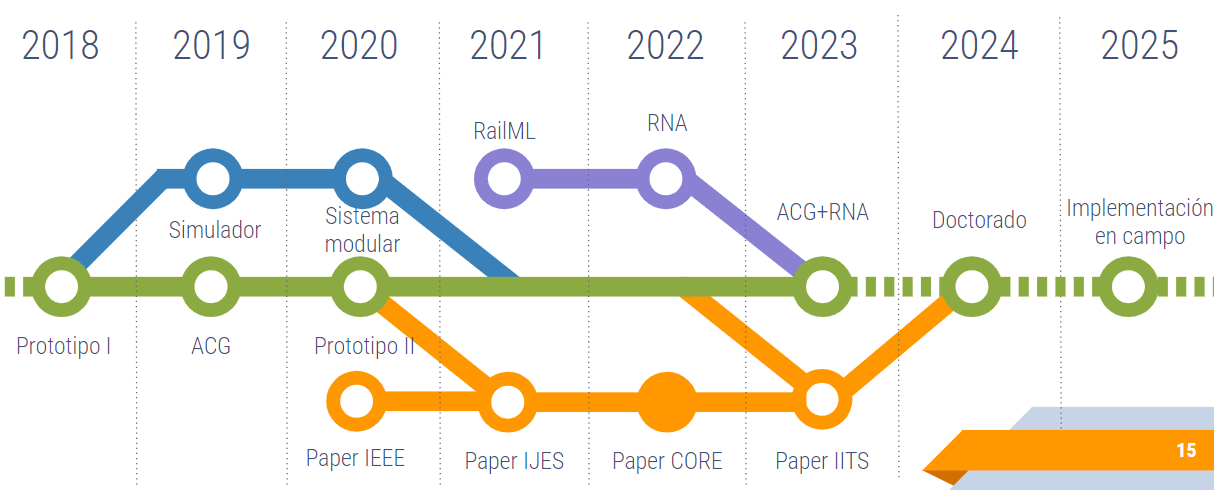
\includegraphics[width=1\textwidth]{Figuras/HojaDeRuta}
        \centering\caption{Trabajos realizados e hitos del proyecto.}
        \label{fig:contexto}
    \end{figure}

    En el año 2018 GICSAFe desarrolló un monitor de barreras ferroviarias instalado en la línea Roca, proyecto que ganó el premio Innnovar 2018 [REF] y permitió ganar experiencia en el área ferroviaria. Desde 2018 se tuvieron varias reuniones con diferentes funcionarios y profesionales de Trenes Argentinos. En particular, con la Gerencia de Ingeniería, Gerencia de Seguridad Operacional, Subgerencia de Desarrollo y Normas Técnicas, Subgerencia de Transporte, Gerencia de Señalamiento, entre otros, de los cuales surgió el interés en el desarrollo del presente proyecto. De dichas visitas y otras posteriores se obtuvo la totalidad de las fotografías incluidas en esta memoria. 

    En el marco de la Maestría de sistemas embebidos, culminada en 2020, se desarrollo un primer prototipo de sistema de enclavamiento con código generado automáticamente en base a un modelo de grafos. Los resultados fueron publicados en IEEE Latin American Transaction en 2020 y en International Journal of Embedded Systems en 2021. En simultáneo, el ingeniero Lucas Dórdolo, miembro de GICSAFe, presentó una actualización del sistema monitor de barreras: el sistema modular [REF], que permitió la lectura y transmisión de datos de la red ferroviaria en tiempo real. Adicionalmente, miembros de GICSAFe pertenecientes a UTN-Haedo comenzaron el desarrollo de un simulador de enclavamientos en tiempo real, que permitió resolver varias cuestiones técnicas de la implementación final del sistema de enclavamiento.

    Hacia finales de 2019 se iniciaron reuniones con miembros de la Comisión Nacional de Energía Atómica (CNEA), para integrar el proyecto en sus plataformas de hardware ampliamente testeada en el ámbito de los sistemas críticos. Además del intercambio de conocimientos y la puesta en común de estrategias a utilizar, se aprovechó todo lo posible la amplia experiencia que ellos brindaron a GICSAFe.
    
    A mediados de 2020, ya formalmente inscripto en el doctorado, se comenzó el desarrollo de una librería compatible con railML 3.0, lo cual se incorporó al primer analizador de redes ferroviarias en 2022, cuyos resultados se publicaron en IEEE Transactions on Intelligent Transportation Systems en 2023. La verificación y validación automática del sistema mediante métodos formales es parte del trabajo de doctorado del ingeniero Santiago Germino, iniciado en 2021. La integración de todas estas herramientas se aplicará en un sistema de enclavamientos a ser instalado en una playa de maniobras real en 2025. 
\section{Principios de señalamiento ferroviario}
    \label{sec:principios}
    
    El proceso de diseño del señalamiento requiere reglas claras y bien definidas sobre cuántas señales colocar, dónde colocar cada señal, bajo que condiciones, de qué tipo deben ser las señales, cómo deben orientarse, etc. Lamentablemente, el criterio utilizado a la hora de definir el señalamiento dista de ser uniforme de nación a nación. La obligatoriedad de ciertas señales, la protección de ciertos elementos, el granularidad de la red o incluso el tener las reglas por escrito son factores que cambian al atravesar las fronteras de cada país. Esto implica, claramente, una barrera enorme al tratar de integrar las redes ferroviarias transnacionales, como en el caso Europeo durante formación de la Unión Europea[REF].
    
    Para la realización de este trabajo se optó por recurrir al Instituto de Ingenieros en Señalamiento Ferroviario (IRSE, por sus siglas en inglés) [IRSE] y a la Junta de Normas y Seguridad de la Industria Ferroviaria (RISSB, por sus siglas en inglés) [RISSB]. Los reglamentos de diseño y definiciones de estas organizaciones son aceptadas por una gran cantidad de empresas del sector ferroviario y autoridades de gran peso. Entre ellas, por la agencia de transporte de Nueva Gales del Sur, en Australia (TfNSW, por sus siglás en inglés) [TfNSW]. De ésta última se recopilaron los siguientes principios de diseño ferroviario:
    
    \begin{itemize}
        \item [($P_1$)] Principio de autoridad: el derecho del tren a circular esta limitada a una pequeña porción de la infraestructura.
        \item [($P_2$)] Principio de claridad: las autoridades otorgadas o negadas no deben ser ambiguas. 
        \item [($P_3$)] Principio de anticipación: los conductores de trenes deben ser advertidos de los peligros cercanos con el suficiente tiempo para reaccionar.
        \item [($P_4$)] Principio de granularidad: las rutas deben ser lo mas cortas posibles.
        \item [($P_5$)] Principio de terminalidad: los conductores de trenes deben ser advertidos cuando se encuentren circulando próximos al final de la red.
        \item [($P_6$)] Principio de infraestructura: los conductores de trenes deben ser advertidos de cualquier infraestructura dinámica o estática próxima.
        \item [($P_7$)] Principio de no bloqueo: se debe evitar en todo momento que los trenes bloqueen el acceso a la infraestructura o ramificaciones a otros tresnes, de ser posible.
    \end{itemize}

    La totalidad del análisis realizado en este proyecto se basa en los principios expuestos. Se puede deducir de los mismos que un sistema de señalamiento debe proteger cada elemento ferroviario ($P_1$,$P_5$,$P_6$), en cada dirección posible ($P_3$,$P_7$). Por lo tanto debemos considerar la posibilidad de que cada tramo de vía puede ser transitado en ambos sentidos ($P_2$,$P_4$) . Esto implica a su vez considerar todas las rutas posibles soportadas por la red ferroviaria, y no solamente las necesarias desde un punto de vista logístico.